%%%%%%%%%%%%%%%%%%%%%%%%%%%%%%%%%%%%

\section{Variability in estimates}

%%%%%%%%%%%%%%%%%%%%%%%%%%%%%%%%%%%%

\begin{frame}
\frametitle{}

\begin{center}
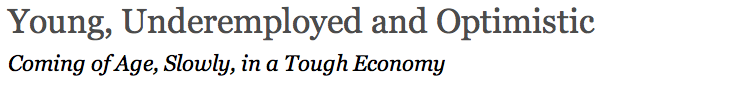
\includegraphics[width=0.95\textwidth]{5-1_var_in_est/figures/pew/pew1} \\
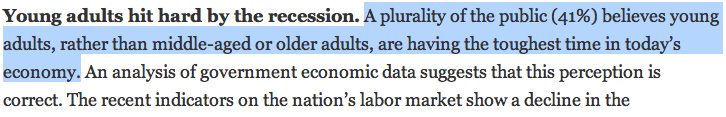
\includegraphics[width=0.95\textwidth]{5-1_var_in_est/figures/pew/pew2} \\
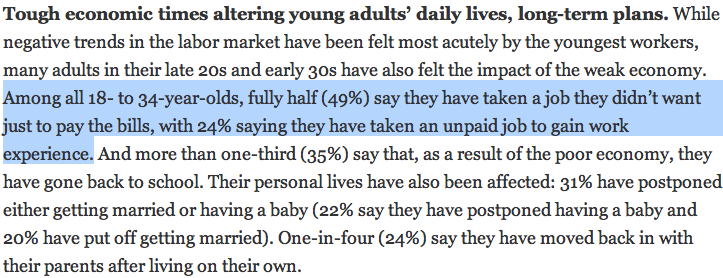
\includegraphics[width=0.95\textwidth]{5-1_var_in_est/figures/pew/pew3}
\end{center}

\ct{\webURL{http://pewresearch.org/pubs/2191/young-adults-workers-labor-market-pay-careers-advancement-recession}}

\end{frame}

%%%%%%%%%%%%%%%%%%%%%%%%%%%%%%%%%%%%

\begin{frame}
\frametitle{Margin of error}

\begin{center}
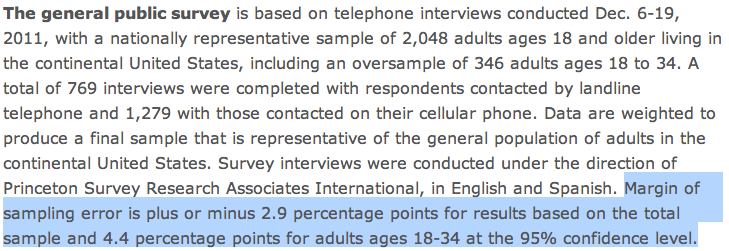
\includegraphics[width=0.95\textwidth]{5-1_var_in_est/figures/pew/pew4}
\end{center}

\begin{itemize}

\item 41\% $\pm$ 2.9\%: We are 95\% confident that 38.1\% to 43.9\% of the public believe young adults, rather than middle-aged or older adults, are having the toughest time in today's economy.


\item 49\% $\pm$ 4.4\%: We are 95\% confident that 44.6\% to 53.4\% of 18-34 years olds have taken a job they didn't want just to pay the bills.

\end{itemize}

\end{frame}

%%%%%%%%%%%%%%%%%%%%%%%%%%%%%%%%%%%%

\begin{frame}
\frametitle{Parameter estimation}

\begin{itemize}

\item We are often interested in \hl{population parameters}.

\item Since complete populations are difficult (or impossible) to collect data on, we use \hl{sample statistics} as \hl{point estimates} for the unknown population parameters of interest.

\item Sample statistics vary from sample to sample.

\item Quantifying how sample statistics vary provides a way to estimate the \hl{margin of error} associated with our point estimate.

\item But before we get to quantifying the variability among samples, let's try to understand how and why point estimates vary from sample to sample.

\end{itemize}

\dq{Suppose we randomly sample 1,000 adults from each state in the US. Would
you expect the sample means of their heights to be the same, somewhat different, or very different?}

\pause

\soln{Not the same, but only somewhat different.}

\end{frame}

%%%%%%%%%%%%%%%%%%%%%%%%%%%%%%%%%%%

\subsection{Application exercise}

%%%%%%%%%%%%%%%%%%%%%%%%%%%%%%%%%%%

\begin{frame}
\frametitle{}

\dq{The following histogram shows the distribution of number of drinks it takes a group of college students to get drunk. We will assume that this is our population of interest. If we randomly select observations from this data set, which values are most likely to be selected, which are least likely?}

\begin{center}
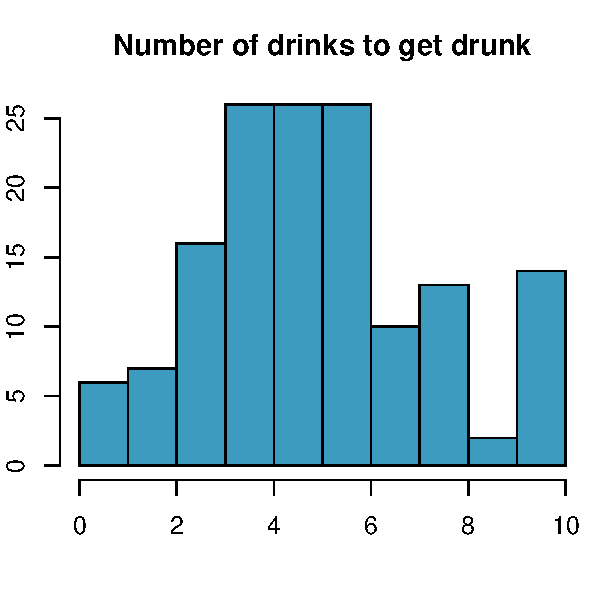
\includegraphics[width=0.5\textwidth]{5-1_var_in_est/figures/no_drinks_drunk/no_drinks_drunk} 
\end{center}

\end{frame}

%%%%%%%%%%%%%%%%%%%%%%%%%%%%%%%%%%

\begin{frame}[fragile]
\frametitle{}

\vspace{-0.25cm}

\dq{Suppose that you don't have access to the population data. In order to estimate the average number of drinks it takes these college students to get drunk, you might sample from the population and use your sample mean as the best guess for the unknown population mean.

\begin{itemize}

\item Sample, with replacement, ten students from the population, and record the number of drinks it takes them to get drunk.

\item Find the sample mean.

\item Plot the distribution of the sample averages  obtained by members of the class.

\end{itemize}
}

\vspace{-0.25cm}

\begin{center}
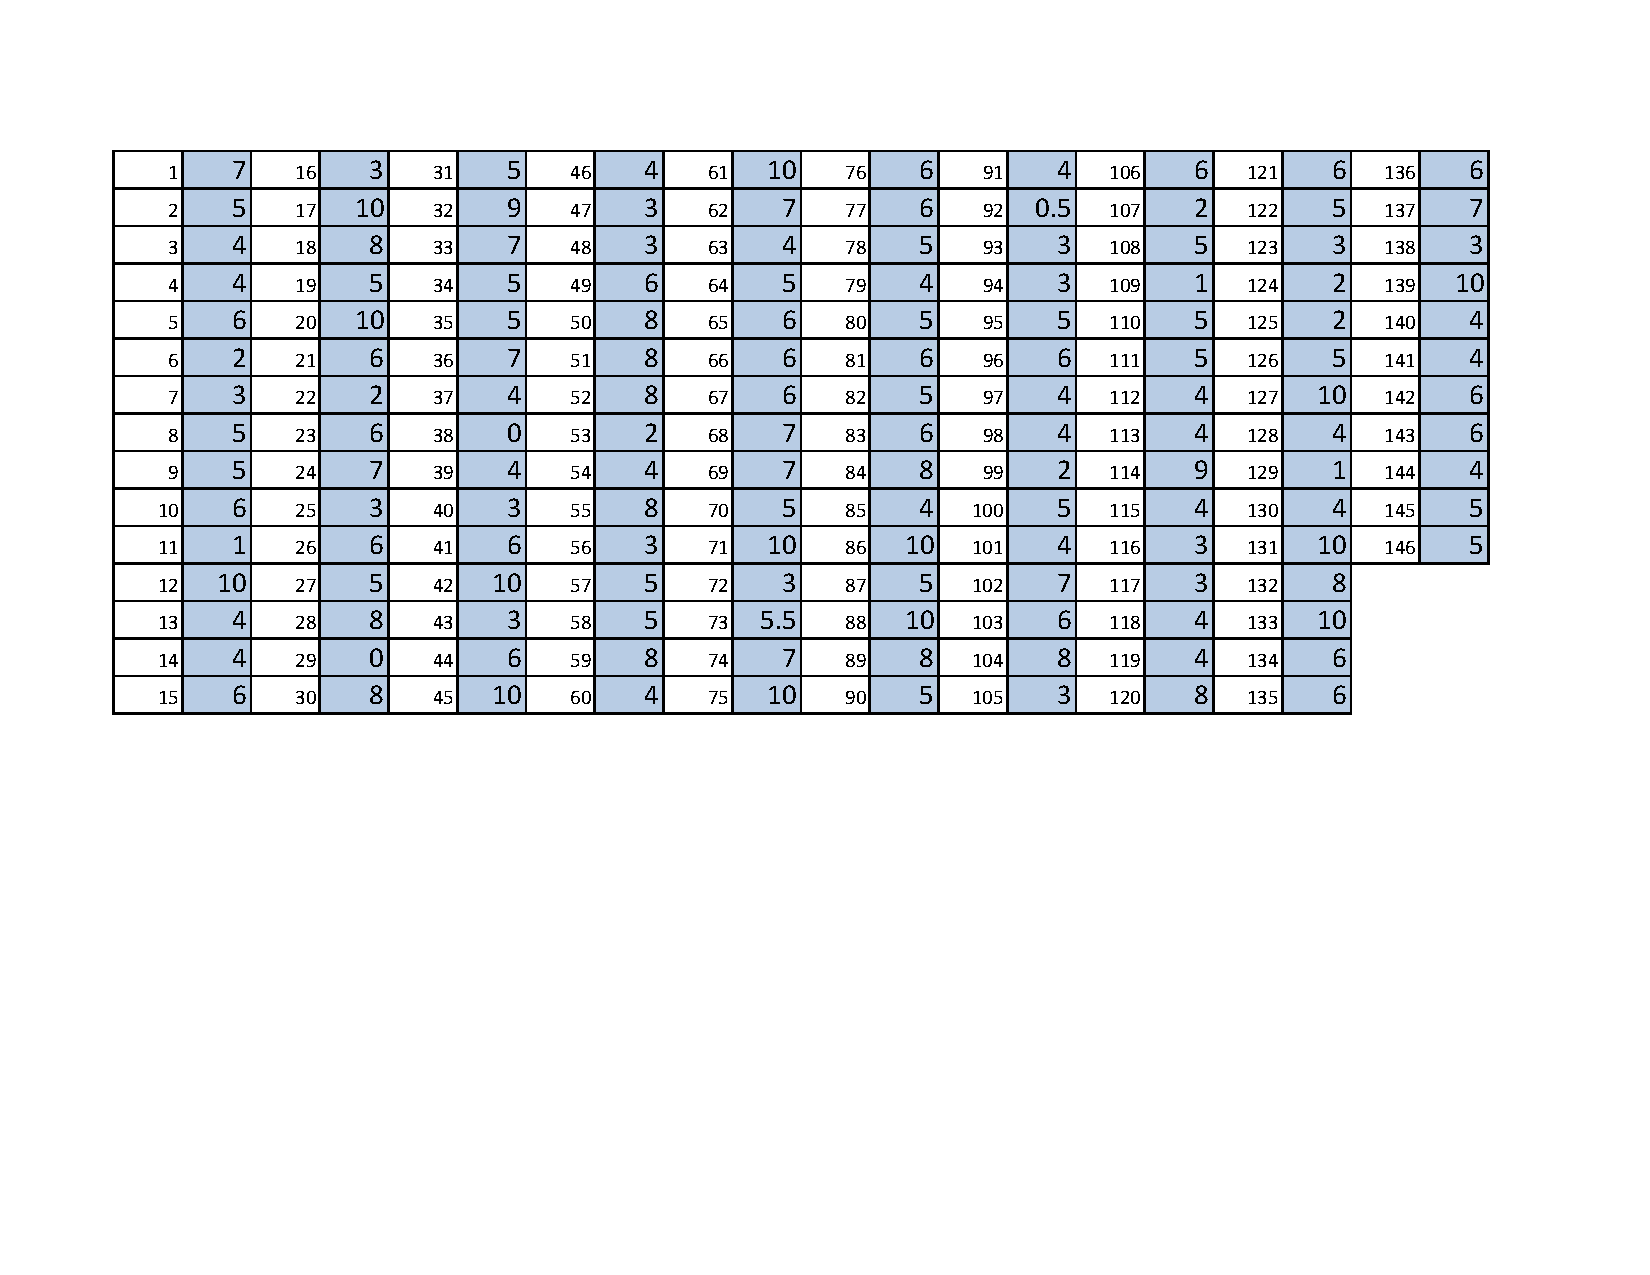
\includegraphics[width=0.8\textwidth]{5-1_var_in_est/figures/no_drinks_drunk/no_drinks_drunk_clean} 
\end{center}

\end{frame}

%%%%%%%%%%%%%%%%%%%%%%%%%%%%%%%%%%%

\begin{frame}[fragile]
\frametitle{}

\dq{Example:} List of random numbers: 59, 121,  88,  46,  58,  72,  82,  81,   5,  10 \\

\begin{center}
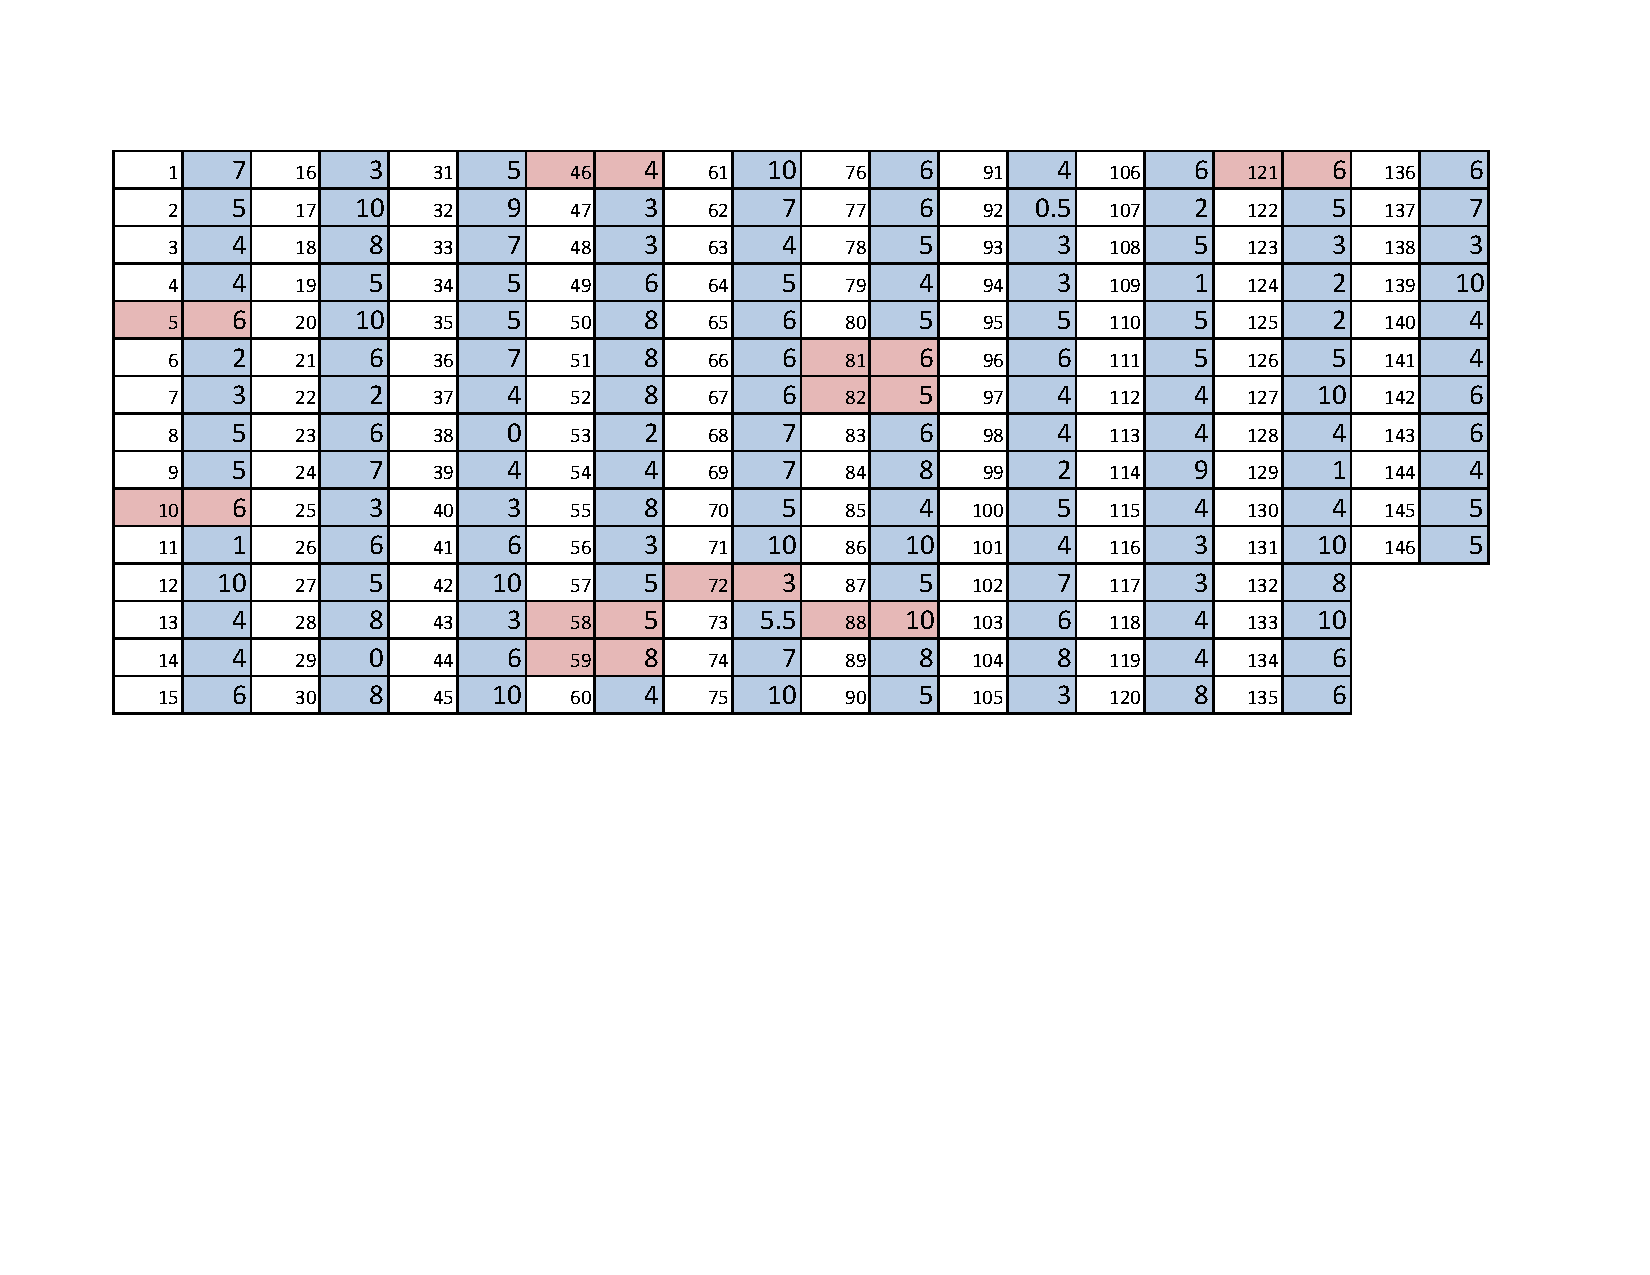
\includegraphics[width=0.9\textwidth]{5-1_var_in_est/figures/no_drinks_drunk/no_drinks_drunk_marked} 
\end{center}

\pause

Sample mean: (8+6+10+4+5+3+5+6+6+6) / 10 = 5.9

\end{frame}

%%%%%%%%%%%%%%%%%%%%%%%%%%%%%%%%%


\begin{frame}[fragile]
\frametitle{Sampling distribution}

What you just constructed is called a \hl{sampling distribution}.

\pause

$\:$ \\
\dq
{What is the shape and center of this distribution? Based on this distribution, what do you think is the true population average?}

$\:$ \\
\soln{\only<3>{
Approximately 5.39, the true population mean.
}}

\end{frame}


%%%%%%%%%%%%%%%%%%%%%%%%%%%%%%%%%%

\subsection{Sampling distributions - via CLT}

%%%%%%%%%%%%%%%%%%%%%%%%%%%%%%%%%%

\begin{frame}
\frametitle{Central limit theorem}

\formula{Central limit theorem}
{The distribution of the sample mean is well approximated by a normal model:
\[ \bar{x} \sim N \pr{ mean = \mu, SE = \frac{\sigma}{\sqrt{n}} }, \]
where SE is represents \hl{standard error}, which is defined as the standard deviation of the sampling distribution. If $\sigma$ is unknown, use $s$.
}

\begin{itemize}

\item It wasn't a coincidence that the sampling distribution we saw earlier was symmetric, and centered at the true population mean.

\item We won't go through a detailed proof of why $SE =  \frac{\sigma}{\sqrt{n}}$, but note that as $n$ increases $SE$ decreases. 
\begin{itemize}
\item As the sample size increases we would expect samples to yield more consistent sample means, hence the variability among the sample means would be lower.
\end{itemize}

\end{itemize}

\end{frame}

%%%%%%%%%%%%%%%%%%%%%%%%%%%%%%%%%%%%

\begin{frame}
\frametitle{CLT - conditions}

Certain conditions must be met for the CLT to apply:

\begin{enumerate}

\item \hlGr{Independence:} Sampled observations must be independent. \\

This is difficult to verify, but is more likely if
\begin{itemize}
\item random sampling/assignment is used, and
\item if sampling without replacement, $n$ $<$ 10\% of the population.
\end{itemize}

\pause

\item \hlGr{Sample size/skew:} Either the population distribution is normal, or if the population distribution is skewed, the sample size is large.\\
\begin{itemize}
\item the more skewed the population distribution, the larger sample size we need for the CLT to apply
\item for moderately skewed distributions $n>30$ is a widely used rule of thumb \\
\end{itemize}

This is also difficult to verify for the population, but we can check it using the sample data, and assume that the sample mirrors the population.

\end{enumerate}

\end{frame}

%%%%%%%%%%%%%%%%%%%%%%%%%%%%%%%%%%%%